% stories_agg.tex — pgfplots port of stories_agg.png.
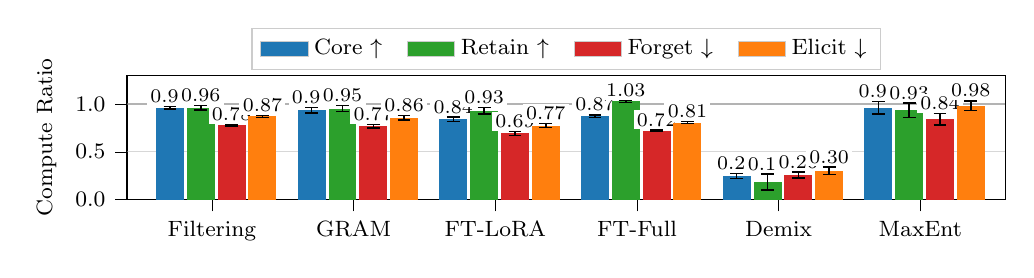
\begin{tikzpicture}
  \pgfplotsset{legend image code/.code={\draw[#1] (0cm,-0.08cm) rectangle (0.22cm,0.08cm);}}

  \definecolor{steelblue31119180}{RGB}{31,119,180}
  \definecolor{forestgreen4416044}{RGB}{44,160,44}
  \definecolor{crimson2143940}{RGB}{214,39,40}
  \definecolor{darkorange25512714}{RGB}{255,127,14}
  \definecolor{darkgray176}{RGB}{176,176,176}
  \definecolor{gray}{RGB}{128,128,128}
  \definecolor{lightgray204}{RGB}{204,204,204}

  \begin{axis}[
  width=0.92\linewidth, height=0.13\linewidth, scale only axis=true,
  tick align=outside, tick pos=left,
  ymin=0, ymax=1.3,
  ytick={0,0.5,1.0},
  yticklabel style={font=\footnotesize, /pgf/number format/.cd, fixed, fixed zerofill, precision=1},
  ylabel={Compute Ratio}, ylabel style={font=\footnotesize},
  xmin=-0.6, xmax=5.6,
  xtick={0,1,2,3,4,5},
  xticklabels={{Filtering},{GRAM},{FT-LoRA},{FT-Full},{Demix},{MaxEnt}},
  xticklabel style={font=\footnotesize},
  xtick style={color=black}, ytick style={color=black},
  legend columns=-1,
  legend style={font=\footnotesize, draw=lightgray204, at={(0.5,1.04)}, anchor=south, /tikz/every even column/.append style={column sep=0.7em}},
  ]
  \addlegendimage{area legend,draw=none,fill=steelblue31119180}
  \addlegendentry{Core $\uparrow$}
  \addlegendimage{area legend,draw=none,fill=forestgreen4416044}
  \addlegendentry{Retain $\uparrow$}
  \addlegendimage{area legend,draw=none,fill=crimson2143940}
  \addlegendentry{Forget $\downarrow$}
  \addlegendimage{area legend,draw=none,fill=darkorange25512714}
  \addlegendentry{Elicit $\downarrow$}
  \addplot [darkgray176, opacity=0.5, line width=0.5pt, forget plot]
  table {%
  -0.6 0.5
  5.6 0.5
  };
  \addplot [gray, opacity=0.6, line width=0.7pt, forget plot]
  table {%
  -0.6 1
  5.6 1
  };
  \draw[draw=none,fill=steelblue31119180] (axis cs:-0.3950,0) rectangle (axis cs:-0.1975,0.96096);
  \draw[black,line width=0.5pt] (axis cs:-0.2963,0.94648)--(axis cs:-0.2963,0.97545);
  \draw[black,line width=0.5pt] (axis cs:-0.3412,0.94648)--(axis cs:-0.2513,0.94648);
  \draw[black,line width=0.5pt] (axis cs:-0.3412,0.97545)--(axis cs:-0.2513,0.97545);
  \node[font=\scriptsize, anchor=south, inner sep=1.2pt, fill=white, fill opacity=1, text opacity=1] at (axis cs:-0.2963,0.97545) {0.96};
  \draw[draw=none,fill=forestgreen4416044] (axis cs:-0.1775,0) rectangle (axis cs:0.0200,0.96211);
  \draw[black,line width=0.5pt] (axis cs:-0.0788,0.93817)--(axis cs:-0.0788,0.98606);
  \draw[black,line width=0.5pt] (axis cs:-0.1237,0.93817)--(axis cs:-0.0338,0.93817);
  \draw[black,line width=0.5pt] (axis cs:-0.1237,0.98606)--(axis cs:-0.0338,0.98606);
  \node[font=\scriptsize, anchor=south, inner sep=1.2pt, fill=white, fill opacity=1, text opacity=1] at (axis cs:-0.0788,0.98606) {0.96};
  \draw[draw=none,fill=crimson2143940] (axis cs:0.0400,0) rectangle (axis cs:0.2375,0.78023);
  \draw[black,line width=0.5pt] (axis cs:0.1388,0.77160)--(axis cs:0.1388,0.78886);
  \draw[black,line width=0.5pt] (axis cs:0.0938,0.77160)--(axis cs:0.1838,0.77160);
  \draw[black,line width=0.5pt] (axis cs:0.0938,0.78886)--(axis cs:0.1838,0.78886);
  \node[font=\scriptsize, anchor=south, inner sep=1.2pt, fill=white, fill opacity=1, text opacity=1] at (axis cs:0.1388,0.78886) {0.78};
  \draw[draw=none,fill=darkorange25512714] (axis cs:0.2575,0) rectangle (axis cs:0.4550,0.87018);
  \draw[black,line width=0.5pt] (axis cs:0.3563,0.85846)--(axis cs:0.3563,0.88191);
  \draw[black,line width=0.5pt] (axis cs:0.3113,0.85846)--(axis cs:0.4012,0.85846);
  \draw[black,line width=0.5pt] (axis cs:0.3113,0.88191)--(axis cs:0.4012,0.88191);
  \node[font=\scriptsize, anchor=south, inner sep=1.2pt, fill=white, fill opacity=1, text opacity=1] at (axis cs:0.3563,0.88191) {0.87};
  \draw[draw=none,fill=steelblue31119180] (axis cs:0.6050,0) rectangle (axis cs:0.8025,0.93746);
  \draw[black,line width=0.5pt] (axis cs:0.7037,0.90808)--(axis cs:0.7037,0.96683);
  \draw[black,line width=0.5pt] (axis cs:0.6587,0.90808)--(axis cs:0.7488,0.90808);
  \draw[black,line width=0.5pt] (axis cs:0.6587,0.96683)--(axis cs:0.7488,0.96683);
  \node[font=\scriptsize, anchor=south, inner sep=1.2pt, fill=white, fill opacity=1, text opacity=1] at (axis cs:0.7037,0.96683) {0.94};
  \draw[draw=none,fill=forestgreen4416044] (axis cs:0.8225,0) rectangle (axis cs:1.0200,0.95221);
  \draw[black,line width=0.5pt] (axis cs:0.9213,0.92239)--(axis cs:0.9213,0.98204);
  \draw[black,line width=0.5pt] (axis cs:0.8762,0.92239)--(axis cs:0.9663,0.92239);
  \draw[black,line width=0.5pt] (axis cs:0.8762,0.98204)--(axis cs:0.9663,0.98204);
  \node[font=\scriptsize, anchor=south, inner sep=1.2pt, fill=white, fill opacity=1, text opacity=1] at (axis cs:0.9213,0.98204) {0.95};
  \draw[draw=none,fill=crimson2143940] (axis cs:1.0400,0) rectangle (axis cs:1.2375,0.76617);
  \draw[black,line width=0.5pt] (axis cs:1.1387,0.74912)--(axis cs:1.1387,0.78321);
  \draw[black,line width=0.5pt] (axis cs:1.0938,0.74912)--(axis cs:1.1837,0.74912);
  \draw[black,line width=0.5pt] (axis cs:1.0938,0.78321)--(axis cs:1.1837,0.78321);
  \node[font=\scriptsize, anchor=south, inner sep=1.2pt, fill=white, fill opacity=1, text opacity=1] at (axis cs:1.1387,0.78321) {0.77};
  \draw[draw=none,fill=darkorange25512714] (axis cs:1.2575,0) rectangle (axis cs:1.4550,0.85540);
  \draw[black,line width=0.5pt] (axis cs:1.3562,0.83124)--(axis cs:1.3562,0.87956);
  \draw[black,line width=0.5pt] (axis cs:1.3113,0.83124)--(axis cs:1.4012,0.83124);
  \draw[black,line width=0.5pt] (axis cs:1.3113,0.87956)--(axis cs:1.4012,0.87956);
  \node[font=\scriptsize, anchor=south, inner sep=1.2pt, fill=white, fill opacity=1, text opacity=1] at (axis cs:1.3562,0.87956) {0.86};
  \draw[draw=none,fill=steelblue31119180] (axis cs:1.6050,0) rectangle (axis cs:1.8025,0.84135);
  \draw[black,line width=0.5pt] (axis cs:1.7037,0.81843)--(axis cs:1.7037,0.86427);
  \draw[black,line width=0.5pt] (axis cs:1.6587,0.81843)--(axis cs:1.7487,0.81843);
  \draw[black,line width=0.5pt] (axis cs:1.6587,0.86427)--(axis cs:1.7487,0.86427);
  \node[font=\scriptsize, anchor=south, inner sep=1.2pt, fill=white, fill opacity=1, text opacity=1] at (axis cs:1.7037,0.86427) {0.84};
  \draw[draw=none,fill=forestgreen4416044] (axis cs:1.8225,0) rectangle (axis cs:2.0200,0.92807);
  \draw[black,line width=0.5pt] (axis cs:1.9212,0.89487)--(axis cs:1.9212,0.96127);
  \draw[black,line width=0.5pt] (axis cs:1.8762,0.89487)--(axis cs:1.9662,0.89487);
  \draw[black,line width=0.5pt] (axis cs:1.8762,0.96127)--(axis cs:1.9662,0.96127);
  \node[font=\scriptsize, anchor=south, inner sep=1.2pt, fill=white, fill opacity=1, text opacity=1] at (axis cs:1.9212,0.96127) {0.93};
  \draw[draw=none,fill=crimson2143940] (axis cs:2.0400,0) rectangle (axis cs:2.2375,0.69181);
  \draw[black,line width=0.5pt] (axis cs:2.1387,0.67070)--(axis cs:2.1387,0.71292);
  \draw[black,line width=0.5pt] (axis cs:2.0938,0.67070)--(axis cs:2.1837,0.67070);
  \draw[black,line width=0.5pt] (axis cs:2.0938,0.71292)--(axis cs:2.1837,0.71292);
  \node[font=\scriptsize, anchor=south, inner sep=1.2pt, fill=white, fill opacity=1, text opacity=1] at (axis cs:2.1387,0.71292) {0.69};
  \draw[draw=none,fill=darkorange25512714] (axis cs:2.2575,0) rectangle (axis cs:2.4550,0.77429);
  \draw[black,line width=0.5pt] (axis cs:2.3563,0.75321)--(axis cs:2.3563,0.79538);
  \draw[black,line width=0.5pt] (axis cs:2.3113,0.75321)--(axis cs:2.4013,0.75321);
  \draw[black,line width=0.5pt] (axis cs:2.3113,0.79538)--(axis cs:2.4013,0.79538);
  \node[font=\scriptsize, anchor=south, inner sep=1.2pt, fill=white, fill opacity=1, text opacity=1] at (axis cs:2.3563,0.79538) {0.77};
  \draw[draw=none,fill=steelblue31119180] (axis cs:2.6050,0) rectangle (axis cs:2.8025,0.87396);
  \draw[black,line width=0.5pt] (axis cs:2.7037,0.86117)--(axis cs:2.7037,0.88675);
  \draw[black,line width=0.5pt] (axis cs:2.6587,0.86117)--(axis cs:2.7487,0.86117);
  \draw[black,line width=0.5pt] (axis cs:2.6587,0.88675)--(axis cs:2.7487,0.88675);
  \node[font=\scriptsize, anchor=south, inner sep=1.2pt, fill=white, fill opacity=1, text opacity=1] at (axis cs:2.7037,0.88675) {0.87};
  \draw[draw=none,fill=forestgreen4416044] (axis cs:2.8225,0) rectangle (axis cs:3.0200,1.02923);
  \draw[black,line width=0.5pt] (axis cs:2.9213,1.01877)--(axis cs:2.9213,1.03968);
  \draw[black,line width=0.5pt] (axis cs:2.8763,1.01877)--(axis cs:2.9663,1.01877);
  \draw[black,line width=0.5pt] (axis cs:2.8763,1.03968)--(axis cs:2.9663,1.03968);
  \node[font=\scriptsize, anchor=south, inner sep=1.2pt, fill=white, fill opacity=1, text opacity=1] at (axis cs:2.9213,1.03968) {1.03};
  \draw[draw=none,fill=crimson2143940] (axis cs:3.0400,0) rectangle (axis cs:3.2375,0.72159);
  \draw[black,line width=0.5pt] (axis cs:3.1387,0.71500)--(axis cs:3.1387,0.72817);
  \draw[black,line width=0.5pt] (axis cs:3.0938,0.71500)--(axis cs:3.1837,0.71500);
  \draw[black,line width=0.5pt] (axis cs:3.0938,0.72817)--(axis cs:3.1837,0.72817);
  \node[font=\scriptsize, anchor=south, inner sep=1.2pt, fill=white, fill opacity=1, text opacity=1] at (axis cs:3.1387,0.72817) {0.72};
  \draw[draw=none,fill=darkorange25512714] (axis cs:3.2575,0) rectangle (axis cs:3.4550,0.80560);
  \draw[black,line width=0.5pt] (axis cs:3.3563,0.79469)--(axis cs:3.3563,0.81651);
  \draw[black,line width=0.5pt] (axis cs:3.3113,0.79469)--(axis cs:3.4013,0.79469);
  \draw[black,line width=0.5pt] (axis cs:3.3113,0.81651)--(axis cs:3.4013,0.81651);
  \node[font=\scriptsize, anchor=south, inner sep=1.2pt, fill=white, fill opacity=1, text opacity=1] at (axis cs:3.3563,0.81651) {0.81};
  \draw[draw=none,fill=steelblue31119180] (axis cs:3.6050,0) rectangle (axis cs:3.8025,0.24780);
  \draw[black,line width=0.5pt] (axis cs:3.7037,0.21826)--(axis cs:3.7037,0.27733);
  \draw[black,line width=0.5pt] (axis cs:3.6587,0.21826)--(axis cs:3.7487,0.21826);
  \draw[black,line width=0.5pt] (axis cs:3.6587,0.27733)--(axis cs:3.7487,0.27733);
  \node[font=\scriptsize, anchor=south, inner sep=1.2pt, fill=white, fill opacity=1, text opacity=1] at (axis cs:3.7037,0.27733) {0.25};
  \draw[draw=none,fill=forestgreen4416044] (axis cs:3.8225,0) rectangle (axis cs:4.0200,0.18302);
  \draw[black,line width=0.5pt] (axis cs:3.9213,0.09844)--(axis cs:3.9213,0.26760);
  \draw[black,line width=0.5pt] (axis cs:3.8763,0.09844)--(axis cs:3.9663,0.09844);
  \draw[black,line width=0.5pt] (axis cs:3.8763,0.26760)--(axis cs:3.9663,0.26760);
  \node[font=\scriptsize, anchor=south, inner sep=1.2pt, fill=white, fill opacity=1, text opacity=1] at (axis cs:3.9213,0.26760) {0.18};
  \draw[draw=none,fill=crimson2143940] (axis cs:4.0400,0) rectangle (axis cs:4.2375,0.25719);
  \draw[black,line width=0.5pt] (axis cs:4.1387,0.22630)--(axis cs:4.1387,0.28807);
  \draw[black,line width=0.5pt] (axis cs:4.0938,0.22630)--(axis cs:4.1837,0.22630);
  \draw[black,line width=0.5pt] (axis cs:4.0938,0.28807)--(axis cs:4.1837,0.28807);
  \node[font=\scriptsize, anchor=south, inner sep=1.2pt, fill=white, fill opacity=1, text opacity=1] at (axis cs:4.1387,0.28807) {0.26};
  \draw[draw=none,fill=darkorange25512714] (axis cs:4.2575,0) rectangle (axis cs:4.4550,0.30161);
  \draw[black,line width=0.5pt] (axis cs:4.3563,0.26185)--(axis cs:4.3563,0.34136);
  \draw[black,line width=0.5pt] (axis cs:4.3113,0.26185)--(axis cs:4.4013,0.26185);
  \draw[black,line width=0.5pt] (axis cs:4.3113,0.34136)--(axis cs:4.4013,0.34136);
  \node[font=\scriptsize, anchor=south, inner sep=1.2pt, fill=white, fill opacity=1, text opacity=1] at (axis cs:4.3563,0.34136) {0.30};
  \draw[draw=none,fill=steelblue31119180] (axis cs:4.6050,0) rectangle (axis cs:4.8025,0.96094);
  \draw[black,line width=0.5pt] (axis cs:4.7038,0.89529)--(axis cs:4.7038,1.02659);
  \draw[black,line width=0.5pt] (axis cs:4.6588,0.89529)--(axis cs:4.7488,0.89529);
  \draw[black,line width=0.5pt] (axis cs:4.6588,1.02659)--(axis cs:4.7488,1.02659);
  \node[font=\scriptsize, anchor=south, inner sep=1.2pt, fill=white, fill opacity=1, text opacity=1] at (axis cs:4.7038,1.02659) {0.96};
  \draw[draw=none,fill=forestgreen4416044] (axis cs:4.8225,0) rectangle (axis cs:5.0200,0.93410);
  \draw[black,line width=0.5pt] (axis cs:4.9212,0.85648)--(axis cs:4.9212,1.01171);
  \draw[black,line width=0.5pt] (axis cs:4.8762,0.85648)--(axis cs:4.9662,0.85648);
  \draw[black,line width=0.5pt] (axis cs:4.8762,1.01171)--(axis cs:4.9662,1.01171);
  \node[font=\scriptsize, anchor=south, inner sep=1.2pt, fill=white, fill opacity=1, text opacity=1] at (axis cs:4.9212,1.01171) {0.93};
  \draw[draw=none,fill=crimson2143940] (axis cs:5.0400,0) rectangle (axis cs:5.2375,0.84033);
  \draw[black,line width=0.5pt] (axis cs:5.1387,0.77921)--(axis cs:5.1387,0.90145);
  \draw[black,line width=0.5pt] (axis cs:5.0938,0.77921)--(axis cs:5.1837,0.77921);
  \draw[black,line width=0.5pt] (axis cs:5.0938,0.90145)--(axis cs:5.1837,0.90145);
  \node[font=\scriptsize, anchor=south, inner sep=1.2pt, fill=white, fill opacity=1, text opacity=1] at (axis cs:5.1387,0.90145) {0.84};
  \draw[draw=none,fill=darkorange25512714] (axis cs:5.2575,0) rectangle (axis cs:5.4550,0.98284);
  \draw[black,line width=0.5pt] (axis cs:5.3563,0.93195)--(axis cs:5.3563,1.03374);
  \draw[black,line width=0.5pt] (axis cs:5.3113,0.93195)--(axis cs:5.4013,0.93195);
  \draw[black,line width=0.5pt] (axis cs:5.3113,1.03374)--(axis cs:5.4013,1.03374);
  \node[font=\scriptsize, anchor=south, inner sep=1.2pt, fill=white, fill opacity=1, text opacity=1] at (axis cs:5.3563,1.03374) {0.98};
  \end{axis}
\end{tikzpicture}
